\documentclass{article}

% Formatting
\usepackage[utf8]{inputenc}
\usepackage[margin=1in]{geometry}
\usepackage[titletoc,title]{appendix}
\usepackage[spanish]{babel}
\usepackage{amsmath,amsfonts,amssymb,mathtools}
\usepackage{graphicx,float}
\usepackage[ruled,vlined]{algorithm2e}
\usepackage{algorithmic}
\usepackage{minted}
\usemintedstyle{borland}
\usepackage{subcaption}
\usepackage{multicol}
\usepackage{listings}
\usepackage{xcolor}
\usepackage{biblatex}
\addbibresource{ref.bib}
\usepackage{minted}



% Title content
\title{Práctica 6 sistema multiagente}
\author{Denisse Leyva}
\date{Marzo 24, 2021}

\begin{document}

\maketitle


\section{Introducción}
Un sistema multiagente es un poco como un autómata celular: hay un conjunto de entidades con estados internos que pueden observar estados de los otros y reaccionar cambiando su propio estado. La diferencia es que un sistema multiagente es un concepto más general y permite que estos agentes se muevan y varíen su vecindad, entre otras cosas. En esta práctica vamos a implementar un sistema multiagente con una aplicación en epidemiología. Los agentes podrán estar en uno de tres estados: susceptibles, infectados o recuperados, esto se conoce como el modelo SIR \cite{Satu_Elisa_Schaeffer}.


\section{Objetivo}
Vacuna con probabilidad $p_{v}$ a los agentes al momento de crearlos de tal forma que están desde el inicio en el estado R y ya no podrán contagiarse ni propagar la infección. Estudia el efecto estadístico del valor de $p_{v}$ en (de cero a uno en pasos de 0.1) el porcentaje máximo de infectados durante la simulación y el momento (iteración) en el cual se alcanza ese máximo \cite{Satu_Elisa_Schaeffer}. 

\section{Código}
En la tarea base se agrego una condición inicial para determinar el porcentaje de vacunados antes que porcentaje de infectados. A demas se automatizó para que se ejecutara por cada porcentaje de vacunación 15 veces en automático. Se utilizó el código base de Schaeffer \cite{Elisa_Schaeffer}. El código completo se encuentra en github \cite{Denisse_Leyva}.

\renewcommand{\listingscaption}{Código}
\begin{listing}[H]
  \begin{minted}[linenos,mathescape,texcl]{clojure}
for va in range(0, 10):
    tt, im = [], []
    pv = va/10
    prim = 0
    for iteraciones in range(15):
        agentes =  pd.DataFrame()
        agentes['x'] = [uniform(0, l) for i in range(n)]
        agentes['y'] = [uniform(0, l) for i in range(n)]
        agentes['dx'] = [uniform(-v, v) for i in range(n)]
        agentes['dy'] = [uniform(-v, v) for i in range(n)]
        agentes['estado'] = ['R' if random() <= pv else 'S' if
                            random() > pi else 'I' for i in range(n)]
        epidemia = []
  \end{minted}
  \label{lst:fibo}
  \caption{Probabilidad de vacunación.}
\end{listing}


\section{Resultados}
Se puede observar en la gráfica que entre mayor porcentaje de vacunación, el máximo número de infectados disminuye, mientras que el momento del pico máximo tiene un rango promedio. El gif para mejor visualización se encuentra en github \cite{Denisse_Leyva}.

\begin{figure}[H]
\centering
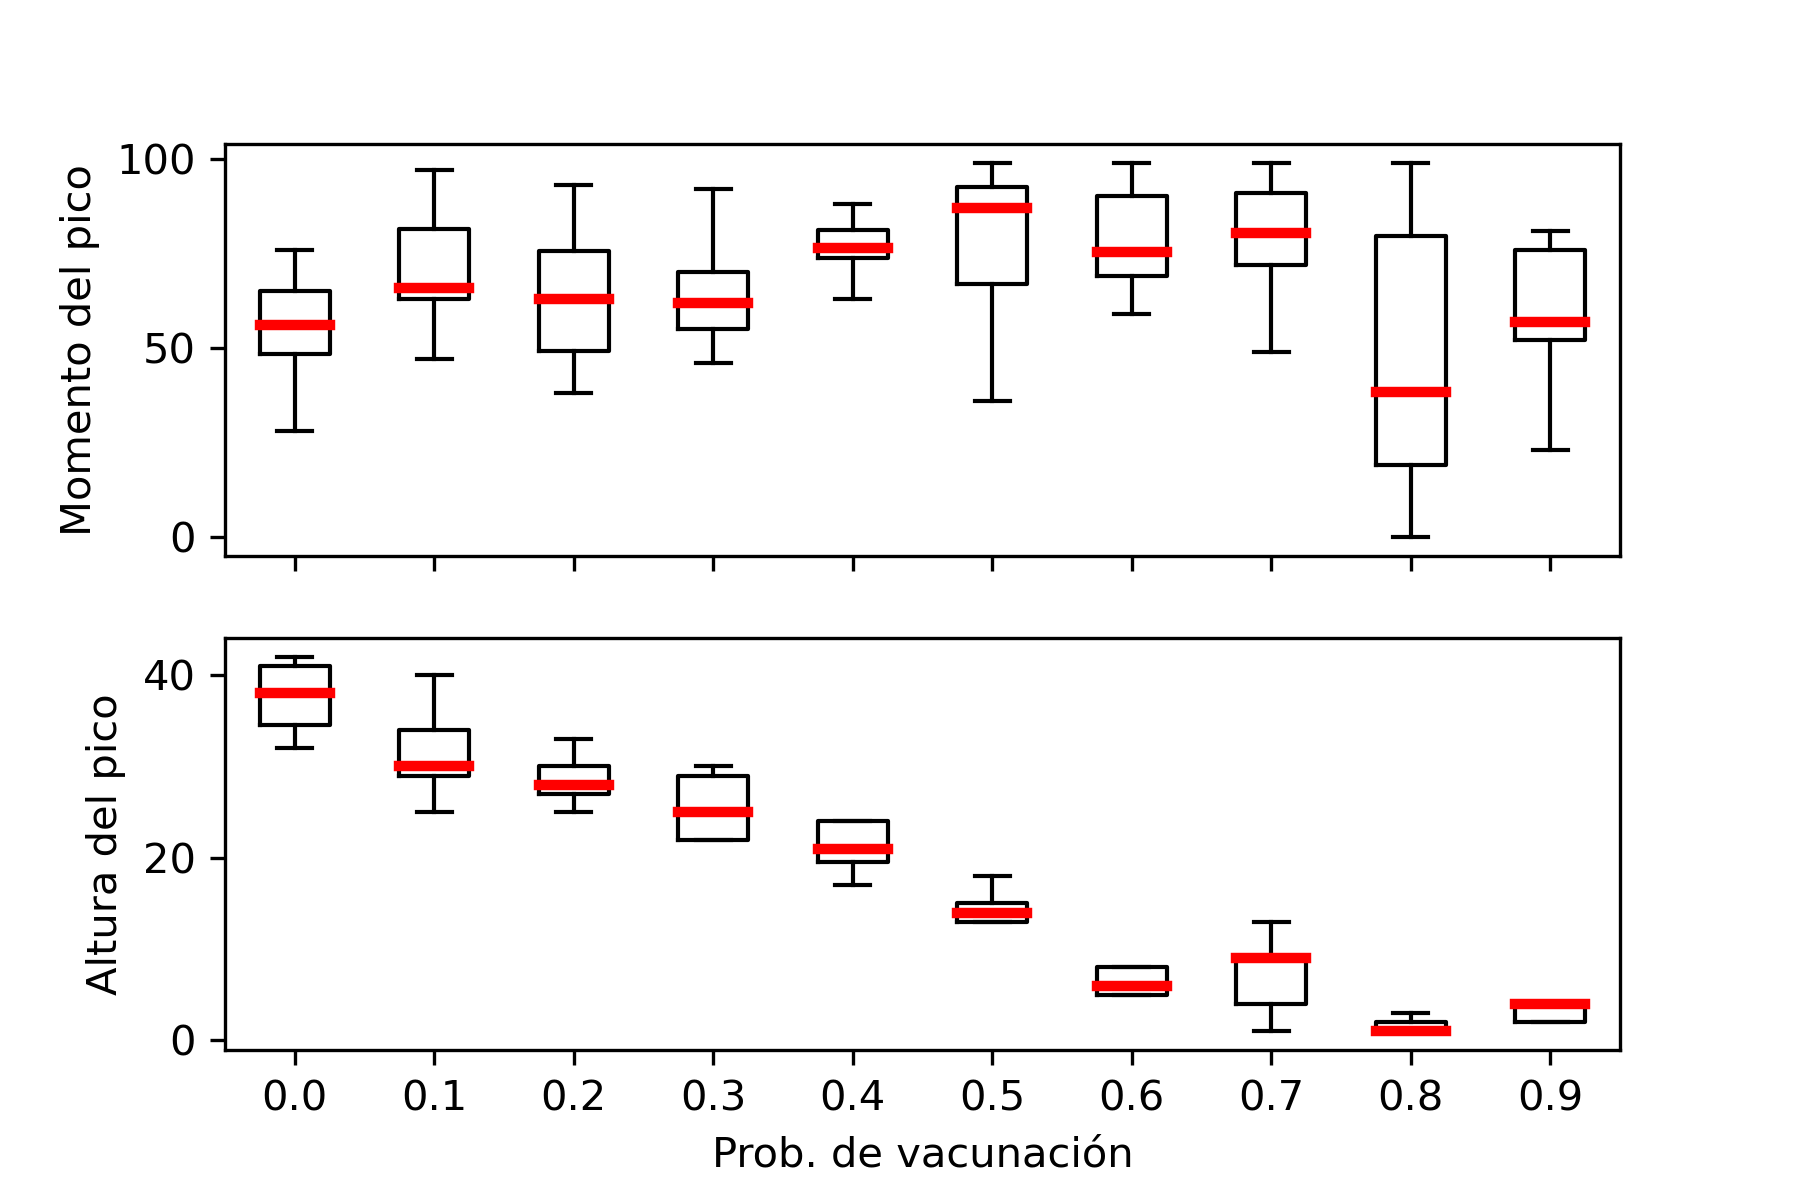
\includegraphics[width=80mm]{p6pg.png}
\caption{\label{fig3}Gráfica de vacunación contra el porcentaje máximo de infectados.}
\end{figure}

\section{Reto 1}
El primer reto es cambiar los patrones de movimiento a que no tengan una trayectoria fija los agentes a que utilice el modelo de punto intermedio aleatorio (inglés: random waypoint model): cada agente tiene una posición meta $(x,y)$ hacia el cual se mueve con una velocidad $v$; al alcanzar (o superar) su meta, elige una nueva meta uniformemente al azar. La velocidad de cada agente es una constante, normalmente distribuido sobre la población de agentes. Examina si surgieron cambios en el efecto de $p_{v}$ por esta modificación \cite{Satu_Elisa_Schaeffer}. El código completo y el gif para mejor visualización se encuentra en github \cite{Denisse_Leyva}.

\renewcommand{\listingscaption}{Código}
\begin{listing}[H]
  \begin{minted}[linenos,mathescape,texcl]{clojure}
agentes =  pd.DataFrame()
agentes['x'] = [uniform(0, l) for i in range(n)]
agentes['y'] = [uniform(0, l) for i in range(n)]
agentes['xi'] = agentes['x']
agentes['yi'] = agentes['y']
agentes['px'] = [uniform(0, l) for i in range(n)]
agentes['py'] = [uniform(0, l) for i in range(n)]
agentes['vpx'] = agentes['x'] < agentes['px']
agentes['vpy'] = agentes['y'] < agentes['py']
agentes['estado'] = ['R' if random() <= pv else 'S' if random() > pi else 'I' for i in range(n)]
vx, vy = False, False
  \end{minted}
  \label{lst:fibo}
  \caption{DataFrame de agentes.}
\end{listing}

\renewcommand{\listingscaption}{Código}
\begin{listing}[H]
  \begin{minted}[linenos,mathescape,texcl]{clojure}
velx = (a.px-a.xi)/v
vely = (a.py-a.yi)/v
x = a.x + velx
y = a.y + vely
if a.vpx:
    if x >= a.px:
        vx = True
else:
    if x <= a.px:
        vx = True

if a.vpy:
    if y >= a.py:
        vy = True      
else:
    if y <= a.py:
        vy = True
x = x if x < l else x - l
y = y if y < l else y - l
x = x if x > 0 else x + l
y = y if y > 0 else y + l
agentes.at[i, 'x'] = x
agentes.at[i, 'y'] = y
if vx and vy:
    agentes.at[i, 'xi'] = a.x
    agentes.at[i, 'yi'] = a.y
    agentes.at[i, 'px'] = uniform(0, l)
    agentes.at[i, 'py'] = uniform(0, l)
    agentes.at[i, 'vpx'] = a.x < a.px
    agentes.at[i, 'vpy'] = a.y < a.py
vx, vy = False, False
  \end{minted}
  \label{lst:fibo}
  \caption{Movimiento de los agentes respecto al punto intermedio aleatorio.}
\end{listing}

\begin{figure}[H]
\centering
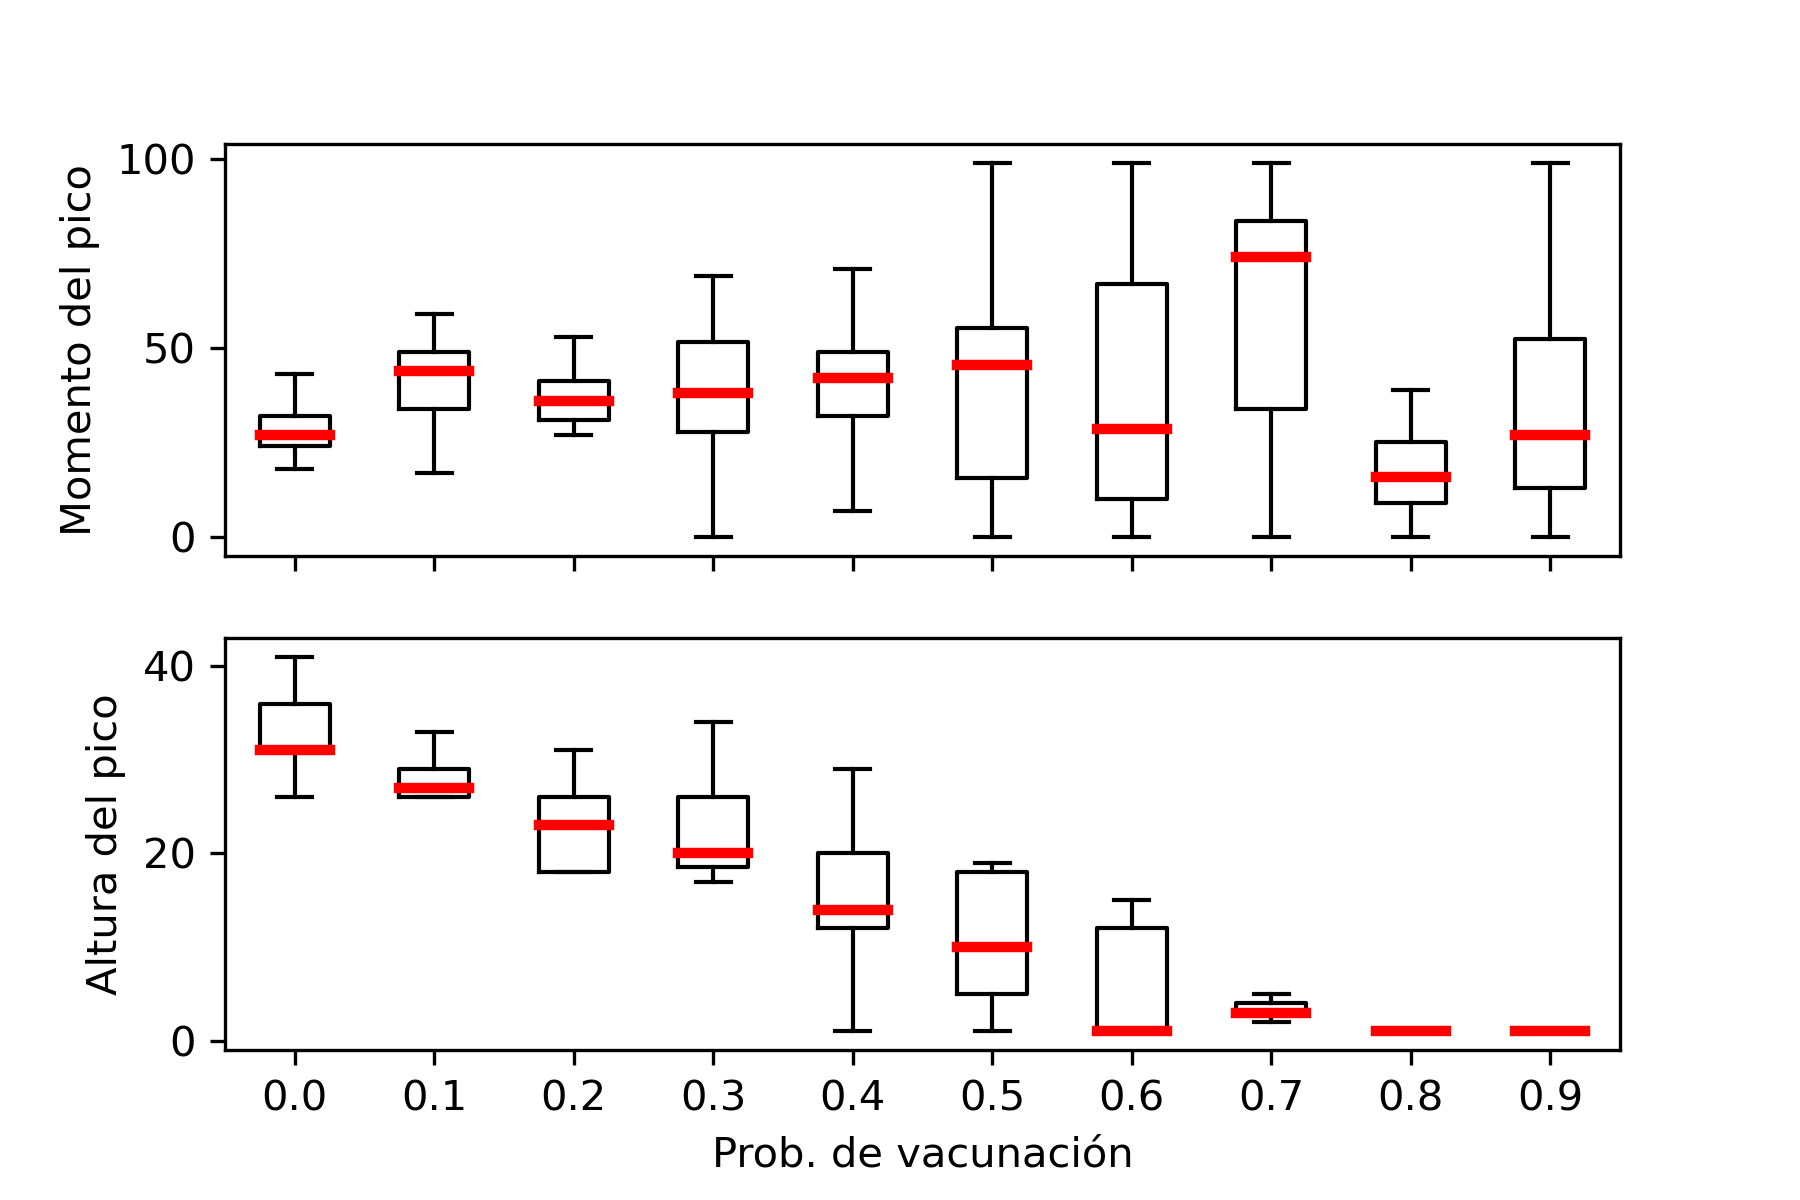
\includegraphics[width=80mm]{p6pgr1.png}
\caption{\label{fig3}Gráfica de vacunación contra el porcentaje máximo de infectados.}
\end{figure}


\section{Reto 2}
En el segundo reto, los agentes tienen amistades: si se encuentran una distancia euclidiana no mayor a $r_{a}$ de un amigo suyo, se disminuye su velocidad a la mitad por $k_{a}$ iteraciones (para saludar a su amigo). Cada par de agentes tiene una amistad con una probabilidad $p_{a}$. Examina nuevamente si surgieron cambios en el efecto de $p_{v}$ por esta modificación, con valores $0 < r_{a} < 1, k_{a} > 1 y 0 < p_{a} << 1$ de tu elección \cite{Satu_Elisa_Schaeffer}. El código completo y gif para mejor visualización se encuentra en github \cite{Denisse_Leyva}.


\renewcommand{\listingscaption}{Código}
\begin{listing}[H]
  \begin{minted}[linenos,mathescape,texcl]{clojure}
# Matriz de amistad
amigos = []
for x in range(n):
    amigo = [] 
    for a in range(n):
        amigo.append(random()<pa)
    amigos.append(amigo)
agentes =  pd.DataFrame()
agentes['x'] = [uniform(0, l) for i in range(n)]
agentes['y'] = [uniform(0, l) for i in range(n)]
agentes['xi'] = agentes['x']
agentes['yi'] = agentes['y']
agentes['px'] = [uniform(0, l) for i in range(n)]
agentes['py'] = [uniform(0, l) for i in range(n)]
agentes['vpx'] = agentes['x'] < agentes['px']
agentes['vpy'] = agentes['y'] < agentes['py']
agentes['estado'] = ['R' if random() <= pv else 'S' if random() > pi else 'I' for i in range(n)]
agentes['amigo'] = [amigos[i] for i in range(n)]
agentes['saludo'] = [False for i in range(n)]
agentes['iteracion'] = [0 for i in range(n)]
  \end{minted}
  \label{lst:fibo}
  \caption{Matriz de amistad y dataframe de agentes.}
\end{listing}

\renewcommand{\listingscaption}{Código}
\begin{listing}[H]
  \begin{minted}[linenos,mathescape,texcl]{clojure}
for mov in range(n):
    b = agentes.iloc[mov]
    if i != mov: #Verificamos que no sea el mismo agente
        if a.amigo[mov]: #Verificamos que uno sea amigo
            dist = sqrt((a.x-b.x)**2 + (a.x-b.x)**2) #Medimos la distancia entre ellos
            if dist <= ra: #Comparamos distancia y cambiamos el saludo a True
                agentes.at[i, 'saludo'] = True
                agentes.at[mov, 'saludo'] = True
if a.saludo: #Verificamos si va a saludar
    if a.iteracion <= ka:
        velx = (a.px-a.xi)/(v*2)
        vely = (a.py-a.yi)/(v*2)
        agentes.at[i, 'iteracion'] += 1
    else:
        agentes.at[i, 'iteracion'] = 0
        agentes.at[i, 'saludo'] = False
        velx = (a.px-a.xi)/v
        vely = (a.py-a.yi)/v
else:
    velx = (a.px-a.xi)/v
    vely = (a.py-a.yi)/v
x = a.x + velx
y = a.y + vely
  \end{minted}
  \label{lst:fibo}
  \caption{Movimiento del agente al momento del saludo.}
\end{listing}


\begin{figure}[H]
\centering
\includegraphics[width=80mm]{.png}
\caption{\label{fig3}Gráfica de vacunación contra el porcentaje máximo de infectados.}
\end{figure}

\printbibliography
\end{document}
